\chapter{Arhitektura i dizajn sustava}
		
		

		Arhitektura sustava je struktura sustava koja sadrži: elemente programa, njihove izvana vidljive karakteristike te odnose među njima.
		Arhitektura sustava se dijeli na tri manja sustava:
		\begin{packed_item}
			\item[$\bullet$] Web poslužitelj
			\item[$\bullet$] Web aplikacija
			\item[$\bullet$] Baza podataka
		\end{packed_item}
		
	
		
		\underbar {\textit {Web preglednik}} je program preko kojega korisnik može pregledavati web-stranice te multimedijalne sadržaje od tih web-stranica. Web-stranica je napisana u kodu koji web preglednik prevodi tako da svatko razumije web-stranicu. Web preglednik također služi kao kanal između korisnika i web poslužitelja.
		
		
		\underbar {\textit {Web poslužitelj}} služi za komunikaciju između klijenta i aplikacije. Ta komunikacija se odvija preko HTTP-a. HTTP je protokol koji se koristi za prijenos podataka na webu. Web poslužitelj također pokreće web aplikaciju i prosljeđuje joj zahtjeve.
		
		
		\underbar {\textit {Web aplikacija}} obrađuje zahtjeve od korisnika, a za pojedine zahtjeve ona pristupa bazi podataka nakon čega se odgovor šalje korisniku putem web poslužitelja te web preglednika u HTML obliku.


		\begin{figure}[H]
			\centering
			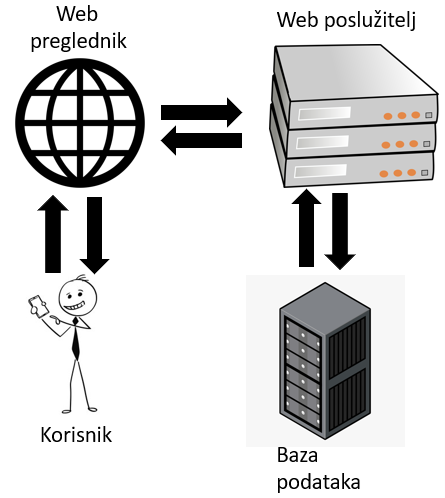
\includegraphics[width=0.75\textwidth]{slike/arhitektura_sustava.PNG} 
			\caption{Arhitektura sustava}
			\label{fig:promjene1} 
		\end{figure}
		
		
		U našemu sustavu za razvoj radnog okvira na poslužiteljskoj strani (backend-u) odlučili smo koristiti \textit {Spring Boot}, a na klijentskoj strani (frontend-u) smo odlučili koristiti \textit {React}. Programske jezike za koje smo se odlučili su \textit {Java} i \textit {JavaScript}.
		
		
		Korišteni razvojni okvir Spring se služi tzv. MVC arhitekturom. Takva arhitektura podrazumijeva sljedeću podjelu:
		\begin{itemize}
			\item[$\bullet$] \textbf{Model}: Središnja komponenta sustava, dohvat te manipulacija podataka
			\item[$\bullet$] \textbf{View}: dostupni razni prikazi podataka (tablično, grafom)
			\item[$\bullet$] \textbf{Controller}: upravlja zahtjevima korisnika te na temelju njih izvodi daljnju interakciju s ostalim komponentama
		\end{itemize}
		
		\vspace{3cm}
		
		Naša web aplikacija koristi višeslojni stil arhitekture. Prednosti višeslojnog stila arhitekture su brojne:
		
		\begin{packed_item}
			\item[$\bullet$] olakšava razvoj programa
			\item[$\bullet$] timovi se mogu raspodijeliti na razvoj zasebnih slojeva arhitekture
			\item[$\bullet$] podjela briga odnosno svaki sloj se mora brinuti za samo svoju zadaću
			\item[$\bullet$] moguće je jednostavno povećanje i poboljšanje sustava
		\end{packed_item}

	
		

		

				
		\section{Baza podataka}
			
			
		
		
		\subsection{Vrsta i implementacija}
		Za modeliranje sustava je korištena relacijska baza podataka, a nju smo implementirati pomoću open-source sustava za upravljanje bazama podataka PostgreSQL. Za izradu dijagrama ER i generiranje relacijske sheme je korišten besplatan online alat ERDplus (https://erdplus.com/) koji je korišten i u sklopu predmeta Baze podataka. 
		
		
		
		\subsection{Glavne komponente baze podataka}
		Baza podataka sastoji se od sljedećih entiteta:
		
		\begin{itemize}
			\item \textbf{Korisnik} \hspace{0.15cm}\textit{Korisnicko\_ime}, \textit{Lozinka}, \textit{Ime}, \textit{Prezime}, \textit{Slika\_osobne}, \textit{IBAN}, \textit{email}, \textit{Uloga}, \textit{stanjeNaRacunu}, \textit{potvrdenVoditelj}, \textit{verificiranKorisnik})
			
			
			\item \textbf{ParkiralisteAutomobili} (\textit{fotografija}, \textit{Naziv}, \textit{Opis}, \textit{CijenaPoSatu}, \textit{ParkiralisteId}) 
			
			\item \textbf{Parking\_mjesto} (\textit{identifikacija}, \textit{Oznaka}, \textit{Slobodno}, \textit{Dostupno}, \textit{ParkiralisteId})
			
			\item \textbf{Voditelj} (\textit{korisnickoIme}, \textit{ParkiralisteId})
			
			\item \textbf{Rezervacija} (\textit{RezervacijaID}, \textit{cijena}, \textit{pocetakRezervacije}, \textit{krajRezervacije}, \textit{RRule}, \textit{KorisnickoIme}, \textit{Identifikacija})
			
			\item \textbf{BicikliMjesto} (\textit{identifikacija}, \textit{BrojMjesta}, \textit{duljina}, \textit{sirina})
		\end{itemize}
		
		
		
			\subsection{Opis tablica}
			

				
			
				
			\textbf{Korisnik:} sadržava sve bitne informacije o registriranim korisnicima u sustavu. Sadrži atribute: ID korisnika, korisničko ime, lozinka, ime, prezime, slika osobne iskaznice, IBAN, email, uloga (enum za 'klijent', 'voditelj', 'administrator') i stanje na računu. Također sadrži dodatne atribute putem kojih pratimo je li korisnik verificirao e-mail (verificiranKorisnik) te, u slučaju uloge=voditelj, je li potvrđen od strane administratora (potvrdenVoditelj). Ovaj entitet je preko korisnickogImena u vezi One-to-Many s entitetom Rezervacija i u One-to-One vezi s entitetom Voditelj.
				\begin{longtblr}[
					label=none,
					entry=none,
					]{
						width = \textwidth,
						colspec={|X[9,l]|X[5,l]|X[20, l]|},
						rowhead = 1,
					}
					\hline \SetCell[c=3]{c}{\textbf{Korisnik}} \\ \hline[3pt]	
					\SetCell{LightGreen} KorisničkoIme & VARCHAR & Jedinstveno korisničko ime \\ \hline
					email & VARCHAR & Email korisnika\\ \hline
					lozinka & VARCHAR & Hash lozinke dobiven s Bcrypt encoderom\\ \hline
					Ime & VARCHAR & Ime korisnika\\ \hline
					Prezime & VARCHAR & Prezime korisnika\\ \hline
					IBAN & VARCHAR &  IBAN korisnika\\ \hline
					slikaOsobne & BYTEA & Byte array slike osobne iskaznice\\ \hline
					Uloga & INT & Enum koji označava ulogu korisnika ('klijent', 'voditelj', 'administrator')\\ \hline
					stanjeNaRacunu & NUMERIC & Decimalni broj koji označava koliko novaca se nalazi u novčaniku \\ \hline
					potvrdenVoditelj & BOOLEAN & Označava je li voditelj potvrđen od strane admina. \\ \hline
					verificiranKorisnik & BOOLEAN & Je li korisnik verificiran preko emaila? \\ \hline
				
				\end{longtblr}
				
				
				
				\noindent\textbf{ParkiralisteAutomobili:} sadrži ključne informacije vezane za parkirališta automobila. Sadrži atribute koje postavlja voditelj parkirališta: fotografija, naziv, opis i cijena po satu. Uz to sadrži i ID parkirališta. Ovaj entitet je u vezi One-to-One s entitetom voditelj putem ID-a parkirališta i One-to-Many vezi s ParkingMjesto preko ID-a parkirališta.
				\begin{longtblr}[
					label=none,
					entry=none
					]{
						width = \textwidth,
						colspec={|X[6,l]|X[6, l]|X[20, l]|}, 
						rowhead = 1,
					}
					\hline \SetCell[c=3]{c}{\textbf{ParkiralisteAutomobili}} \\ \hline[3pt]
					\SetCell{LightGreen}ParkiralisteId & INT & Jedinstveni identifikator parkirališta\\ \hline
					fotografija & BYTEA & Slika parkirališta koju voditelj može priložiti\\ \hline
					Naziv & VARCHAR & Naziv parkirališta\\ \hline
					Opis & VARCHAR & Opis parkirališta\\ \hline
					CijenaPoSatu & NUMERIC & Cijena po satu koju definira voditelj parkirališta\\ \hline
				
				\end{longtblr}
				
				\noindent\textbf{Parking\_mjesto:} predstavlja informacije o pojedinačnim parkirnim mjestima unutar parkirališta za automobile. U ovu tablicu ćemo unijeti početne informacije o mjestima za automobile koje smo dobili od overpass API-ja.  Sadrži atribute kao što su identifikacija i koordinate (duljina, širina) koje ćemo dobiti pozivom overpassAPI-a. (@id i "coordinates" iz GeoJSON-a dobivenog pozivom overpassAPI-a), oznaka parkirnog mjesta, informacija o dostupnosti koju postavlja voditelj i slobodnom statusu parkirnog mjesta te ID parkirališta kojem pripada. U U vezi je Many-to-One s entitetom "ParkirališteAutomobili" putem ID-a parkirališta i One-to-many s entitetom Rezervacija putem identifikacije parking mjesta.
				\begin{longtblr}[
					label=none,
					entry=none
					]{
						width = \textwidth,
						colspec={|X[6,l]|X[6, l]|X[20, l]|}, 
						rowhead = 1,
					}
					\hline \SetCell[c=3]{c}{\textbf{Parking\_mjesto}} \\ \hline[3pt]
					\SetCell{LightGreen}identifikacija & VARCHAR & Identifikacija mjesta koje generira overpassAPI koji generira overpassAPI. \newline Npr. "node/11310562209" \\ \hline
					Oznaka & VARCHAR & Oznaka ili broj parkirnog mjesta\\ \hline
					Duljina & NUMERICAL & Označuje duljinu (longitude) \\ \hline
					Sirina & NUMERICAL & Označuje širinu (longitude)\\ \hline
					Slobodno & BOOLEAN & Je li mjesto slobodno ili nije\\ \hline
					Dostupno & BOOLEAN & Je li voditelj učinio mjesto dostupnim\\ \hline
					\SetCell{LightBlue}ParkiralisteId & INT & Jedinstveni identifikator parkirališta \newline (ParkiralisteAutomobili.ParkiralisteID)\\ \hline
				
				\end{longtblr}
				
				\noindent\textbf{Voditelj:} sadrži informacije o voditeljima parkirališta. Povezuje voditelja sa parkiralištem. Ima vezu s One-to-one s entitetima Korisnik i ParkirališteAutomobila.
				\begin{longtblr}[
					label=none,
					entry=none
					]{
						width = \textwidth,
						colspec={|X[6,l]|X[6, l]|X[20, l]|}, 
						rowhead = 1,
					}
					\hline \SetCell[c=3]{c}{\textbf{Voditelj}} \\ \hline[3pt]
					
					\SetCell{LightBlue}korisnickoIme & VARCHAR & Jedinstveno korisničko ime \\ \hline
					\SetCell{LightBlue}ParkiralisteId & INT & Jedinstven ID parkinga \newline(ParkiralisteAutomobili.ParkiralisteID)\\ \hline
				\end{longtblr}
				
				\noindent\textbf{Rezervacija:} sadrži informacije o parking rezervacijama koje su napravili korisnici. Uz cijenu i timestampe za pocetak i kraj rezervacije sadrži i string (TEXT) RRule kojim se definira učestalost ponavljanja rezervacije. Taj string se može parsirati pa generirati instance ponavljućih rezervacija. Ovaj entitet ima vezu Many-to-One s entitetom Korisnik putem jedinstvenog korisničkog imena. Također, ima vezu Many-to-One s entitetom "ParkingMjesto" putem lokacije parkirnog mjesta.
				\begin{longtblr}[
					label=none,
					entry=none
					]{
						width = \textwidth,
						colspec={|X[9,l]|X[6,l]|X[19, l]|},  % Adjust the width for the second column
						rowhead = 1,
					}
					\hline \SetCell[c=3]{c}{\textbf{Rezervacija}} \\ \hline[3pt]
					\SetCell{LightGreen}RezervacijaID & INT & Jedistven identifikator rezervacije\\ \hline
					Cijena & NUMERIC & Ukupna cijena rezervacije\\ \hline
					pocetakRezervacije & TIMESTAMP & Jedinstveni identifikator rezervacije \\ \hline
					krajRezervacije & TIMESTAMP & Ukupna cijena rezervacije\\ \hline
					RRule & TEXT & String koji će definirati učestalost ponavljanja rezervacije na osnovi formata iCalendar (RFC 5545) (ako je NULL onda je jednokratna)\\ \hline
					\SetCell{LightBlue}korisnickoIme & INT & Jedinstveno korisničko ime\\ \hline
					\SetCell{LightBlue}identifikacija & INT & Jedinstven identifikator parkirnog mjesta \newline \newline\\ \hline
				\end{longtblr}
				
				\noindent\textbf{BicikliParking:} unosimo početne informacije o biciklističkim mjestima. Pošto se parkirališta za bicikle ne mogu rezervirati niti se naplaćuju, ovaj entitet je odvojen od ostatka sustava. Sadrži atribute: koordinate (širina i duljina) te identifikaciju koje dobivamo pozivom overpassAPI-ja. Duljina je prva vrijednost, a širina druga vrijednost u coordinates arrayu. \\ Npr. "coordinates": [16.0166069 (duljina), 45.8387721 (sirina)]
				\begin{longtblr}[
					label=none,
					entry=none
					]{
						width = \textwidth,
						colspec={|X[9,l]|X[6,l]|X[19, l]|},  % Adjust the width for the second column
						rowhead = 1,
					}
					\hline \SetCell[c=3]{c}{\textbf{BicikliParking}} \\ \hline[3pt]
					\SetCell{LightGreen}identifikacija & VARCHAR & Jedistven identifikator mjesta (@id iz GeoJSON-a)\\ \hline
					brojMjesta & INT & Broj dostupnih mjesta na parkingu za bicikle\\ \hline
					duljina & NUMERICAL & (longitude) prva vrijednost u "coordinates" nizu\\ \hline
					sirina & NUMERICAL & (latitude) druga vrijednost u "coordinates nizu"\\ \hline
					
					
				\end{longtblr}
				
				\subsection{Dijagram baze podataka}
				\begin{figure}[H]
					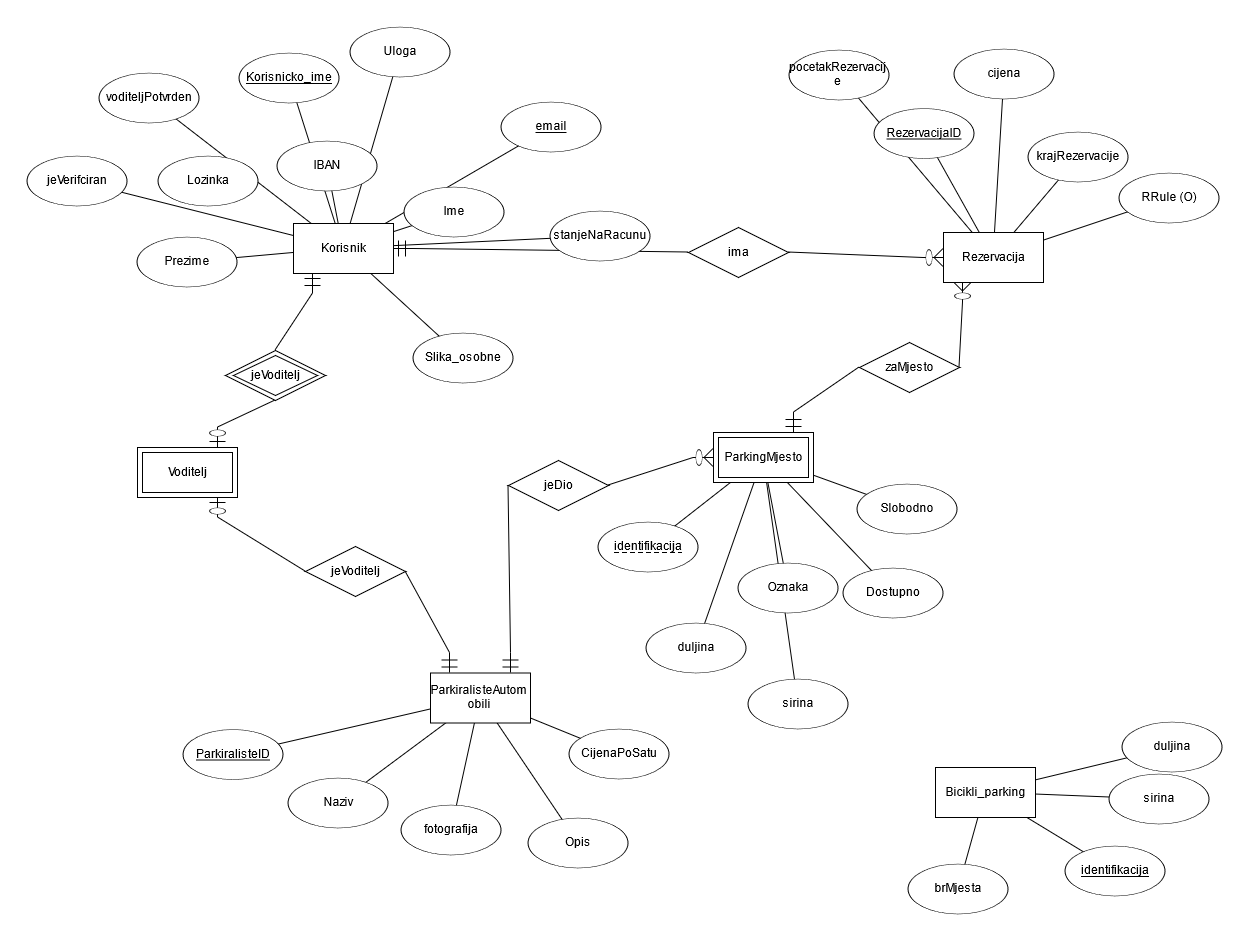
\includegraphics[width=\textwidth]{slike/erldiagram.PNG} %veličina slike u odnosu na originalnu datoteku i pozicija slike
					\centering
					\caption{E-R dijagram baze podataka}
					\label{fig:erldijagram}
				\end{figure}
				
				\begin{figure}[H]
					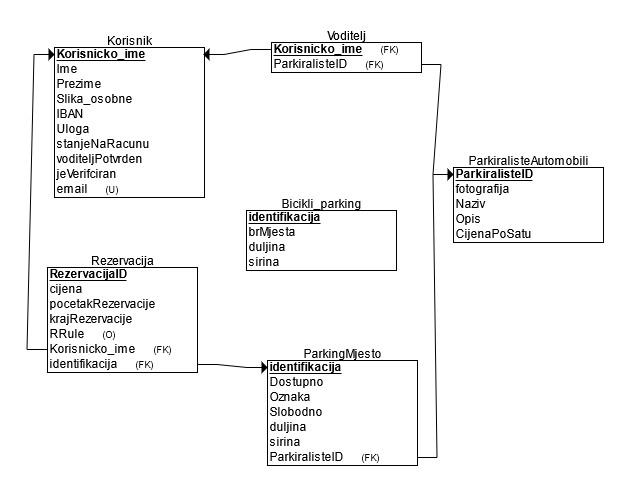
\includegraphics[scale=0.7]{slike/rlcdiagram.PNG} %veličina u odnosu na širinu linije
					\caption{Relacijska shema}
					\label{fig:relshema} %label mora biti drugaciji za svaku sliku
				\end{figure}
				
				
				
				
				
			
			
			
			
			
			\eject
			
			
		\section{Dijagram razreda}
		
			\begin{figure}[H]
				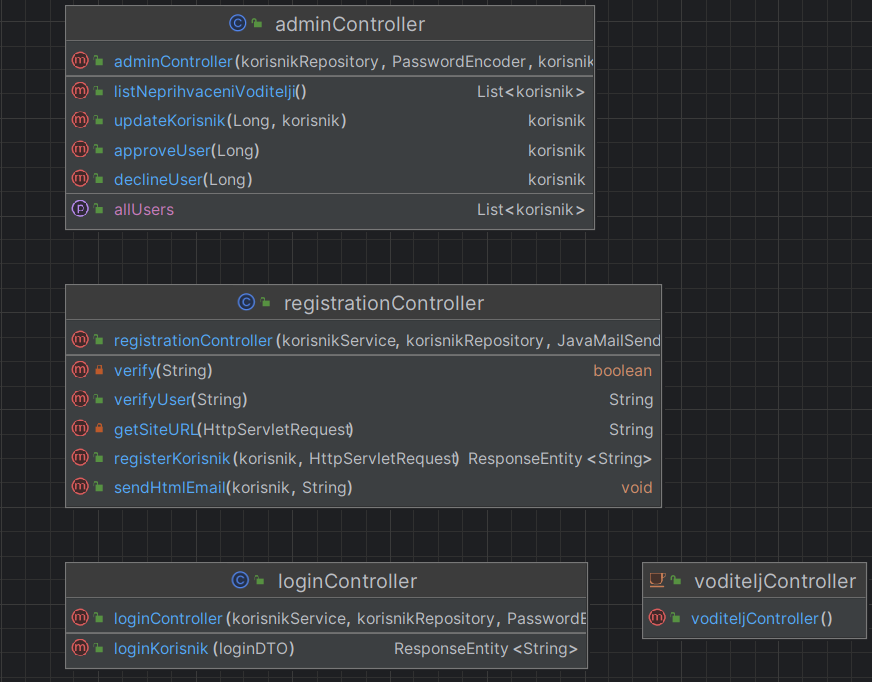
\includegraphics[width=\textwidth]{slike/dijagram_razred1.PNG} %veličina slike u odnosu na originalnu datoteku i pozicija slike
				\centering
				\caption{Dijagram razreda}
%				\label{fig:dijagramrazreda1}
			\end{figure}
			
			\begin{figure}[H]
				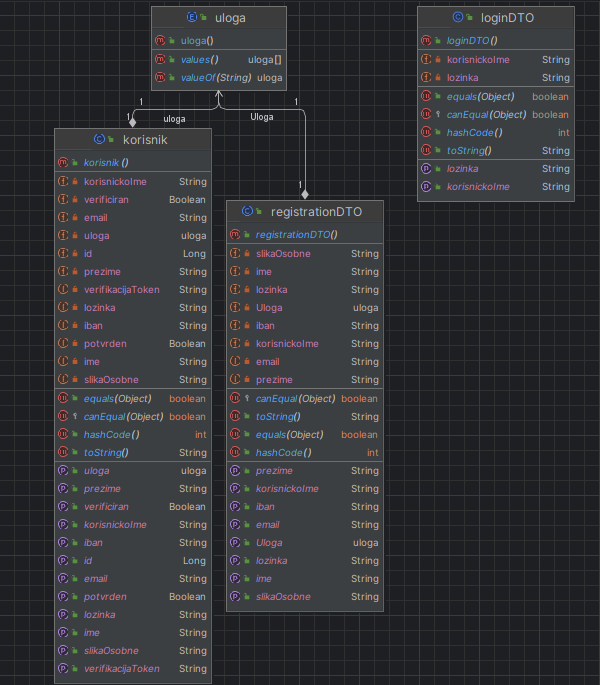
\includegraphics[width=\textwidth]{slike/dijagram_razred2.PNG} %veličina slike u odnosu na originalnu datoteku i pozicija slike
				\centering
				\caption{Dijagram razreda}
				\label{fig:dijagramrazreda2}
			\end{figure}
			
			\begin{figure}[H]
				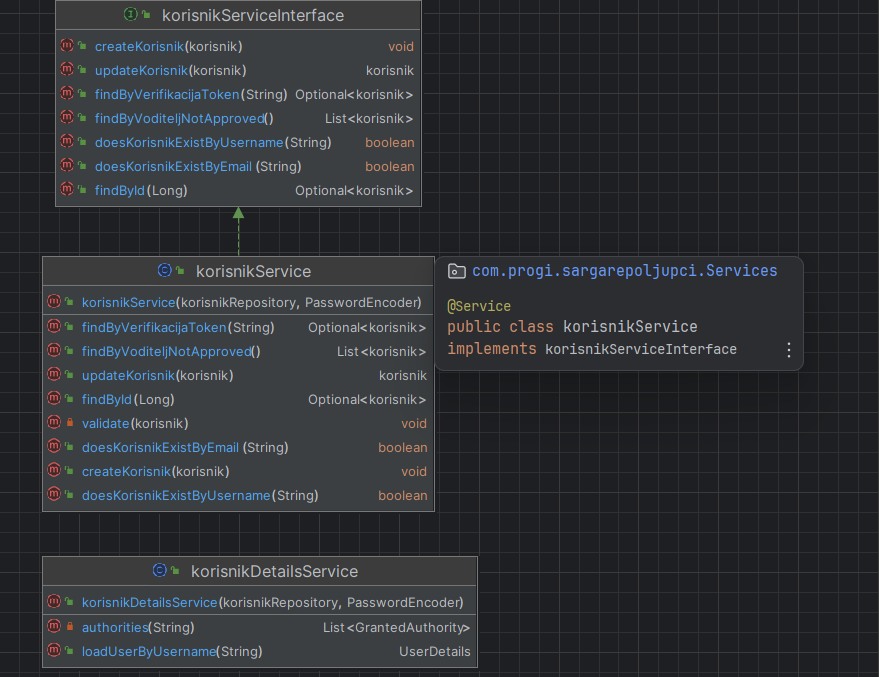
\includegraphics[width=\textwidth]{slike/dijagram_razred3.PNG} %veličina slike u odnosu na originalnu datoteku i pozicija slike
				\centering
				\caption{Dijagram razreda}
				\label{fig:dijagramrazreda3}
			\end{figure}
			
			
			
			\eject
		
		\section{Dijagram stanja}
			
			
			\textbf{\textit{dio 2. revizije}}\\
			
			\textit{Potrebno je priložiti dijagram stanja i opisati ga. Dovoljan je jedan dijagram stanja koji prikazuje \textbf{značajan dio funkcionalnosti} sustava. Na primjer, stanja korisničkog sučelja i tijek korištenja neke ključne funkcionalnosti jesu značajan dio sustava, a registracija i prijava nisu. }
			
			
			\eject 
		
		\section{Dijagram aktivnosti}
			
			\textbf{\textit{dio 2. revizije}}\\
			
			 \textit{Potrebno je priložiti dijagram aktivnosti s pripadajućim opisom. Dijagram aktivnosti treba prikazivati značajan dio sustava.}
			
			\eject
		\section{Dijagram komponenti}
		
			\textbf{\textit{dio 2. revizije}}\\
		
			 \textit{Potrebno je priložiti dijagram komponenti s pripadajućim opisom. Dijagram komponenti treba prikazivati strukturu cijele aplikacije.}